\section{Цель работы}

Экспериментальное исследование линейных разветвленных
резистивных цепей с использованием методов наложения, эквивалентного
источника и принципа взаимности.

\section{Приборы и материалы}

\begin{itemize}
    \item мультиметр;
    \item набор резисторов;
    \item соединительные провода.
    \item Схема для исследования, изображенная на рис. \ref*{fig:scheme_1}.
\end{itemize}

\begin{figure}[!h]
    \centering
    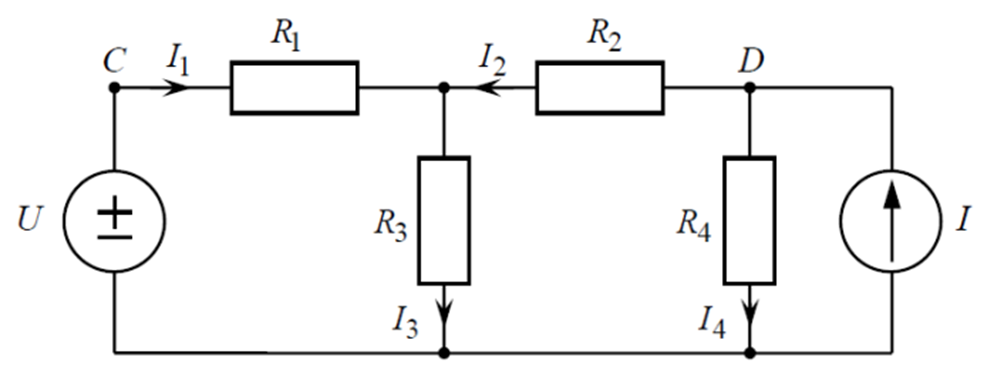
\includegraphics{scheme_1.png}
    \caption{Схема для исследования}
    \label{fig:scheme_1}
\end{figure}

$R_1 = R_2 = 1,5$ кОм, $R_3 = R_4 = 3$ кОм.
